Time-series prediction of a neural model relies on the input history of equally distributed samples.
The LSTM model is a recurrent neural network designed to solve the vanishing gradient problem by remembering/preserving the long dependencies~\cite{rasifaghihi_predictive_2020}.
The cells inside the model act as memory units to preserve the dependence.
Therefore, the output is closely dependent on the previous input samples.
Unlike the normal RNN and the more modern version - GRU, LSTM has a more complicated structure constructed from several logical gates~\cite{LSTM_Hochreiter1997}.
It is the most widely used type of model.
\ifthenelse {\boolean{thesis}}
{
Chapter~\ref{} at section~\ref{} and \mbox{Figure~\ref{}} provide a summary of the LSTM cell logic.
} 
{
\mbox{Figure~\ref{fig:LSTM-cell2}} provides a summary of the cell logic.
It utilises three gates: forget $f_t$, input $i_t$ and output $o_t$, \mbox{Equation~\ref{eq:LSTM-gates2}}.
The decisions are based around sigmoid $\sigma$ function~\ref{eq:sigmoid2}.
With default $tanh$ as activation function, \mbox{Equation~\ref{eq:LSTM-output2}} describes the procedure for cell state update and further propagation.
Output variables $h_t$ and $c_t$ represent memory cell output and the cell state at timestamp $t$.
\begin{equation}
    \sigma(x) = \frac{1}{1+e^{-x}}
    \label{eq:sigmoid2}
\end{equation}
\begin{figure}[htbp]
    \centering
    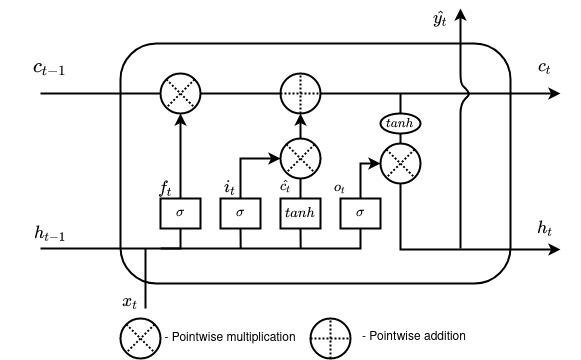
\includegraphics[width=\linewidth]{II_Body/LSTM/images/LSTM.jpg}
    \caption{Long Short-Term Memory Cell}
    \label{fig:LSTM-cell2}
\end{figure}
\begin{equation}
    \begin{split}
        f_t &= \sigma \left(W_f \left[h_{t-1}, x_t \right] + b_f \right) \\
        i_t &= \sigma \left(W_i \left[h_{t-1}, x_t \right] + b_i \right) \\
        o_t &= \sigma \left(W_o \left[h_{t-1}, x_t \right] + b_o \right) \\    
    \end{split}
    \label{eq:LSTM-gates2}
\end{equation}
\begin{equation}
    \begin{split}
        c_t &= f_t c_{t-1}+i_t \times tanh \left(W_c \left[h_{t-1}, x_t \right] + b_c \right) \\
        h_t &= o_t*tanh \left(c_t \right)
    \end{split}
    \label{eq:LSTM-output2}
\end{equation}
}

%
%
The LSTM model has been used widely in stock-price prediction or weather forecasting.
However, unlike State of Charge estimation, which commonly uses $V$, $I$ and $T$ as inputs, those methods utilise the output feature as an input to the subsequent prediction to propagate results further and calculate the time before a critical event occurrence.
Besides, methods like weather forecasting a weak ahead are not limited by lacking output data, since the searched criteria is always known or will be known.
Contrarily, a True State of Charge of a battery cannot be determined and verified against previously made predictions without additional battery modelling techniques. (not to mention of having it integrated into Electric Vehicle.)
(As oppose to the SoC estimate, where getting true values require battery cycler capable with set of ) 
%%%%%%%%%%%
%Unlike the charge estimation, which can only output a single value based on a history of samples, they are not limited to... Therefore does not require the output as input since the truth will become known in due time.

%
%
The best way to utilise the performance of the stateless LSTM model is through training with a data windowing technique.
The NN model will receive a fixed set of equally distributed time samples at each time prediction.
Every next forecast will shift the time window by a constant step $s$, until all possible combinations of time slices go through the model.
That approach is referred to as a stateless model, which sees dependencies over input samples only, rather than preserving every received input, like in stateful implementations.
It also allows the order of the windows to be shuffled to avoid overfitting
Since no dropout was applied before models output a set of strategies strategies has been applied to vary learning rate and rollback before early stopping to assist the fitting process.
\ifthenelse {\boolean{thesis}}
{
Chapter~\ref{} at sections~\ref{}and~\ref{} provide an explanation to those two methods, which already proven to be useful at training SoC models.
} 
{
    \textbf{TODO: EIther import that content from previos article, reference it, or redo entirely}
}
As a result, a NN model will learn dependency between a fixed amount of equally distributed time samples $n$ and yet independent from the order of the inputs.
\mbox{Figure~\ref{fig:Windowing}} demonstrates how the input dataset is constructed and ordered into a 3-dimensional dataset, with 4 features, 500 timestamps and around 110k* samples to fit on.
Due to the size of the windows, equivalent to 8 and quoter minutes of a discharge process, no batching mechanism has been used to reduce computational load and avoid 4-dimensional matrix management.


%
%
The mean and standard deviation has normalised all data to speed up the training process.
The normalisation constant from training input samples must be used for validation and testing sets to ensure the right trends.
The state of charge will be narrowed between 0 and 1 to represent the percentage charge in 2 decimal numbers.
\mbox{Table~\ref{tab:params}} highlights the parameters required to define the initial model, where $s$ defines output step size.
Use of a $\sigma$ function as an output justified by the charge normalisation between 0 and 1.
\begin{table}[ht]
    \renewcommand{\arraystretch}{1.3}
    \caption{Model structure and parameters}
    \centering
    \label{tab:params}
    \resizebox{\columnwidth}{!}{
    \begin{tabular}{ l l l }
        \hline\hline \\[-4mm]
        Input     & $shape= \left( 1,500,4 \right)$ & $batch=1 $  \\
        \hline
        LSTM      & $activation= 'tanh'$ & $units=510$  \\
        \hline
        Dropout   & $0.0$ &   \\
        \hline
        Output    & $activation= \sigma\left(s, 1 \right)$ &   \\
        \hline\hline
    \end{tabular}
    }
\end{table}

%
%
\ifthenelse {\boolean{thesis}}
{
The optimisation algorithm for the fitting process has been defined by regular Adam from the previous chapter, \mbox{Algorithm~\ref{}}, with the corresponding hyperparameters, \mbox{Table~\ref{}}.

}
{
The optimisation algorithm for the fitting process has been defined by Adam, \mbox{Algorithm~\ref{alg:copyAdam}}, with the following hyperparameters, \mbox{Table~\ref{tab:newM-params}}.
%\textcolor{red}{Try to use Robust Adam instead, because why the hell not since I lost one month of my life to implement that cursed algorithm from Javids miss-typed notes? Complete this section with details as per Gareth Javid's implementation if RoAdam will be able to produce a faster fitting.}
\begin{algorithm}\captionsetup{labelfont={sc,bf}, labelsep=newline}
    \caption{Adaptive Moment Estimation (Adam) optimisation}
    \begin{algorithmic}[1]
        \STATE \textbf{Number of input samples} \\ $N\gets length(\textit{input data})$\\
        \STATE \textbf{Size of windows} \\ $S\gets length(V_{i..n})$\\
        \STATE \textbf{Output steps} \\ $O\gets length(V_{i..n})$\\
        \STATE Input: $x_n = [V_{i..n}, I_{i..n}, T_{i..n}, SoC_{(i-1)..(n-1))}]$ \\
         - Shape: $X = (N, S, 4)$
        \STATE Output:$y_n = [SoC_{(n-o)..n}] - $Shape:$Y = (N, O, 1)$
        \STATE Define Loss function: $L$ \\
                Get hyperparameters: $\alpha, \beta_1, \beta_2, \epsilon$
        \WHILE{$W_t \text{ not converge}$}
        \STATE $t \gets t+1$
        \STATE $g_t \gets \nabla_W L_t (W_{t-1})$ \COMMENT{Obtain gradient}
        \STATE $m_t \gets \beta_1 m_{t-1}+(1-\beta_1) g_t $ \COMMENT{$1_{st}$ moment calculation}
        \STATE $\upsilon_t \gets \beta_2 \upsilon_{t-1}+ \left(1-\beta_2 \right)g^2_t $ \COMMENT{$2_{nd}$ moment calculation \label{alg:Adam-Line-2Moment}}
        \STATE $\hat{m_t} \gets \frac{m_t}{1-\beta^t_1}$ \COMMENT{Corrected $\hat{m_t}$}
        \STATE $\hat{\upsilon_t} \gets \frac{\upsilon_t}{1-\beta^t_2} $ \COMMENT{Corrected $\hat{\upsilon_t}$}
        \STATE $W_t \gets W_{t-1}- \alpha \frac{\hat{m_t}}{\sqrt{\hat{\upsilon_t}}+\epsilon} $ \COMMENT{Update parameters}
        \ENDWHILE
    \end{algorithmic}
    \label{alg:copyAdam}
\end{algorithm}
\begin{table}[htbp]
    \renewcommand{\arraystretch}{1.3}
    \caption{Optimiser specific hyperparameters}
    \centering
    \label{tab:newM-params}
    \resizebox{\columnwidth}{!}{
    \begin{tabular}{ l l l l }
        \hline\hline \\[-4mm]
        $\alpha$ & $\beta_1 $ & $\beta_2$ & $\epsilon$ \\
        \hline
        $0.001$ & $0.9$ & $0.999$ & $10^{-8}$ \\% 0.0000001
        \hline\hline
    \end{tabular}
    }
\end{table}
}